
\documentclass[a4paper,12pt]{article} % тип документа


% Русский язык
\usepackage[T2A]{fontenc} % кодировка
\usepackage[utf8]{inputenc} % кодировка исходного текста
\usepackage[english,russian]{babel} % локализация и переносы


% Математика
\usepackage{amsmath,amsfonts,amssymb,amsthm,mathtools}


\usepackage{wasysym}

%Заговолок
\author{Талашкевич Даниил Александрович}

\title{Бонусная задача. Неделя № 6}

\date{\today}

\begin{document}

\maketitle
\thispagestyle{empty}

\newpage
\setcounter{page}{1}
\begin{center}
\itshape
\bfseries
{ \Large БОНУСНАЯ ЗАДАЧА № 6}
\end{center}

{\bf (*) }а) Доказать теорему Форда-Фалкерсона; б)доказать теорему Кенига.
\begin{center}
\bfseries
{\Large Решение: }
\end{center}

а) Теорема Форда-Фалкерсона -- величина максимального потока в графе путей равна величине пропускной способности его минимального разреза.

Для начало проясним, что такое поток:\\
Пусть дана транспортная сеть $N=(V,E)$ с источником $s\in V$, стоком $t\in V$ и пропускными способностями $c$.\\
Величиной поток называется сумма потоков из источника $ |f|=\sum _{{v\in V}}f_{{sv}}$

А разрез графа в свою очередь:\\
Разрез графа в задачах о потоке — такая пара множеств вершин $(S,T)$, что:

1)$S\cup T=V$, где $V$ -- множество вершин графа

2)$S\cap T=\emptyset$

3)$s\in S,t\in T$, где $s$ -- исток, $t$ -- сток.\\
Если неформально, то разрез графа — множество рёбер, удаление которых делит граф на два изолированных подграфа, один из которых, в частности, может быть отдельным узлом.

А величиной разреза называется сумма пропускных способностей таких рёбер $(i, j)$, что $i\in S,j\in T$.

{\bf Доказательство:}  любой поток$f(u,v)$ между вершинами $t$ и $s$  по определению меньше или равен величине любого сечения. Пусть дан некоторый поток$f$ и некоторое сечение. Величина данного потока складывается из величин «грузов», перевозимых по всем возможным путям из вершины $s$(source, источник) в $t$(sink, сток) . Каждый такой путь обязан иметь общее ребро с данным сечением. Так как по каждому ребру сечения суммарно нельзя перевести «груза» больше, чем его пропускная способность($ f(u,v)\leqslant c (u, v) $), поэтому сумма всех грузов меньше или равна сумме всех пропускных способностей рёбер данного сечения ($\sum\limits_{i = 1}^{|E|}c_i$). 
\begin{flushright}
\begin{large}
\textbf {Утверждение доказано. }
\end{large}
\end{flushright}

\newpage
б)Теорема Кёнига -- в любом двудольном графе число рёбер в наибольшем паросочетании равно числу вершин в наименьшем вершинном покрытии.



{\bf Доказательство:} Пусть задан двудольный граф $ G=(X,Y,E)$, а   
\hspace{66mm}$M$ -- наибольшее паросочетание в $G$.

Сначала рассмотрим случай, когда паросочетание $M$ насыщает все вершины доли $X$, то есть размер паросочетания $M$ равен $|X|$. Очевидно, что вся доля $X$ является вершинным покрытием$^{*}$ в графе $G$, следовательно, она является и наименьшим вершинным покрытием, и в этом случае утверждение теоремы выполняется.

(*) Вершинное покрытие -- это множество его вершин $S$, такое, что, у каждого ребра графа хотя бы один из концов входит в вершину из $S$.\\

Иначе возьмём все вершины доли $X$, не насыщенные паросочетанием $M$, и запустим из них обход в ширину($\ast$) по следующему правилу:


($\ast$)Поиск в ширину -- один из методов обхода графа. Пусть задан граф $G=(V,E)$ и выделена исходная вершина $s$. Алгоритм поиска в ширину систематически обходит все ребра $G$ для «открытия» всех вершин, достижимых из $s$, вычисляя при этом расстояние (минимальное количество рёбер) от $s$ до каждой достижимой из $s$ вершины. Алгоритм работает как для ориентированных, так и для неориентированных графов.)


1. Слева направо переходим только по рёбрам, не входящим в $M$ (будем называть их чёрными).

2. Справа налево переходим только по рёбрам, входящим в $M$ (будем называть их голубыми).

Пусть $X^{+}$ и $Y^{+}$ — подмножества вершин левой и правой доли, посещённых во время обхода, а $X^{-}$ и $ Y^{-}$ — соответственно, подмножества не посещённых вершин (см. рисунок 1).\\

\begin{center}
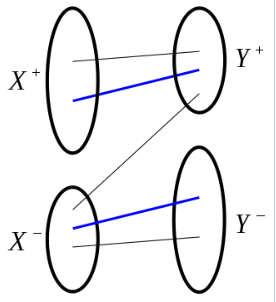
\includegraphics[scale=1]{6 2}

Рис. 1
\end{center}

Между множествами $X^{+}$ и $ Y^{-}$ нет чёрных рёбер, поскольку иначе во время обхода мы бы посетили вершины из множества $Y^{-}$. По аналогичной причине, между множествами $X^{-}$ и $Y^{+}$ нет голубых рёбер.

Докажем, что между множествами $ X^{+}$ и $Y^{-}$ нет также и голубых рёбер. От противного, пусть такое ребро $\{x^{+},y^{-}\}$ есть. Вершина $x^{+}$ не могла являться стартовой для обхода в ширину, поскольку она насыщена паросочетанием $M$. Следовательно, обход в ширину пришёл в $x^{+}$ из какой-то вершины $y^{+}$ по голубому ребру, что означает, что вершине $x^{+}$ инцидентны два голубых ребра $\{x^{+},y^{-}\}$ и $\{x^{+},y^{+}\}$. Но это невозможно, поскольку голубые рёбра образуют паросочетание.

Следовательно, любое ребро графа $G$ инцидентно или вершине из $X^{-}$ или вершине из $Y^{+}$, то есть $X^{-}\cup \ Y^{+}$ является вершинным покрытием. Покажем, что все вершины в $X^{-}\cup \ Y^{+}$ насыщены паросочетанием $M$. Для вершин из $X^{-}$ -- это очевидно, поскольку все ненасыщенные вершины левой доли по построению лежат в $X^{+}$. Если в$Y^{+}$ есть ненасыщенная вершина, то существует $M$ --чередующая цепь, заканчивающаяся в ней, что противоречит тому, что паросочетание $M$ является наибольшим. Теперь осталось вспомнить, что между множествами $X^{-}$ и $Y^{+}$ нет рёбер из $M$, то есть каждому ребру паросочетания инцидентна в точности одна вершина из вершинного покрытия $ X^{-}\cup \ Y^{+}$. Следовательно, $|M|=|X^{-}\cup \ Y^{+}|$, и вершинное покрытие $X^{-}\cup \ Y^{+}$ является наименьшим.



\begin{flushright}
\begin{large}
\textbf {Доказано }
\end{large}
\end{flushright}


\end{document}


